% vim:set shiftwidth=2 tabstop=2 expandtab:
% \pagebreak[4]
% \hspace*{1cm}
% \pagebreak[4]
% \hspace*{1cm}
% \pagebreak[4]

\chapter{Uniform Convergence Rates for a Class of Martingales} \la{chap:1}
\ifpdf
    \graphicspath{{Chapter1/Chapter1Figs/PNG/}{Chapter1/Chapter1Figs/PDF/}{Chapter1/Chapter1Figs/}}
\else
    \graphicspath{{Chapter1/Chapter1Figs/EPS/}{Chapter1/Chapter1Figs/}}
\fi
For a class of martingales, this chapter provides a framework on the uniform consistency with broad applicability. The main condition imposed is only related to the conditional variance of the martingale. Our results not only  provide sharp convergence rate, but also the optimal range for the uniform convergence to be held. This chapter also considers the uniform upper and lower  bound estimates for a functional of Harris recurrent Markov chain, which  are of independent interests. These results will be useful for the study of sample covariance functional and sample average functional appear in a nonlinear cointegration model.

\section{Introduction}
Let $(u_k, x_k)$ with $x_k=(x_{k1},..., x_{kd}), d\ge 1,$ be a sequence of random vectors. A common functional of interests $S_{1n}(x)$ of
$(u_k, x_k)$ is defined by
\be
  S_{1n}(x) =\sum_{k=1}^n u_k g[(x_k+x)/h], \quad x\in R^d,\la {eqn:1:in1}
\ee
where $h=h_n\to 0$ is a certain sequence of positive constants and $g$ is a real function on $R^d$. Such functionals arise in nonparametric estimation problems, where $g$ may be a kernel function $K$ or a squared kernel function $K^{2}$ and the
sequence $h$ is the bandwidth used in the nonparametric regression.


The uniform convergence of $S_{1n}(x)$ in the situation that the $(u_k, x_k)$ satisfy certain stationary conditions was studied in many articles. \cite{liero1989}, \cite{peligrad1992} and \cite{nzedoukhan2004} considered the uniform convergence over a fixed compact set, while \cite{masry1996}, \cite{bosq1998} and \cite{fanyao2003} gave uniform results over an unbounded set. These work mainly focus on random sequence $x_t$ which satisfies different types of mixing conditions. Investigating a more general framework, \cite{andrews1995} gave result on kernel estimate when the data sequence is near-epoch dependent on another underlying mixing sequence. More recently, \cite{hansen2008} provided a set of general uniform consistency results, allowing for stationary strong mixing multivariate data with infinite support, kernels with unbounded support and general bandwidth sequences. \cite{kristensen2009} further extended Hansen's results to the heterogenous dependent case under $\alpha$-mixing condition. Also see \cite{wuhuanghuang2010} for kernel estimation in general time series settings.


In comparison to the extensive results where the  $x_k$ comes from a stationary time series data, there is little investigation on the the uniform convergence of $S_{1n}(x)$ for the $x_k$ being a non-stationary time series. In this regard, \cite{gaolitjostheim2011} derived strong and weak consistency results for the case where the $x_k$ is a null-recurrent Markov chain. \cite{wangwang2012} worked  with partial sum processes of the type $x_k=\sum_{j=1}^k\xi_j$ where $\xi_j$ is a general linear process. While the rate of convergence   in \cite{gaolitjostheim2011} is sharp,  they impose the independence between $u_k$ and $x_k$. Using a quite different method, \cite{wangwang2012} allowed for the endogeneity between $u_k$ and $x_k$, but their results hold  only for the $x$ being in a fixed compact set.

The aim of this chapter is to present a general uniform consistency  result for $S_{1n}(x)$ with broad applicability. As a framework,  our  assumption on the $x_t$ is only related to the conditional variance of the  martingale, that is, $ \sum_{t=1}^n g^2[(x_t+x)/h]$. See Assumption \ref{assump:1:highLevel} in Section \ref{sec:1:martingale}.
This of course is a ``high level" condition, but it in fact is quite natural which holds true for many interesting and important examples, including stationary mixing time series, stationary  iterated random function and Harris  recurrent Markov chain. See Sections \ref{sec:1:identification} and \ref{sec:1:markov} for the identification of Assumption \ref{assump:1:highLevel}. This condition also holds true for $I(1)$ processes with innovations being a linear process, but the identification is complicated and requires quite different techniques. We will report related work in Chapter \ref{chap:2} and \ref{chap:3}. It should be mentioned that our work on the uniform upper and lower  bound estimation for a functional of Harris recurrent Markov chain is of independent interests.


This chapter is organized as follows. Our main results are presented in next section, which includes the establishment of a framework on the uniform convergence for a class of martingale and uniform upper and lower  bound estimation for a functional of Harris recurrent Markov chain. All proofs are postponed to Section \ref{sec:1:proof}. 


\section{Uniform convergence for a class of martingales} \la{sec:1:martingale}
We make use of the following assumptions in the development of  uniform convergence for the $S_{1n}(x)$ defined by (\ref {eqn:1:in1}).
Recall $x_k=(x_{k1},..., x_{kd})$ where $ d\ge 1$ is an integer.

\begin{assump} \la{assump:1:martingale}
  $\{u_t, {\mathcal F}_t\}_{t\ge 1}$ is a martingale difference, where  ${\mathcal F}_t=\si (x_1, ..., x_{t+1}, u_1,...,u_t)$, satisfying $ \sup_{t\ge 1}E(|u_t|^{2p}\mid {\mathcal F}_{t-1})<\infty, a.s., $ for some $p\ge 1$ specified  in Assumption \ref{assump:1:bandwidth} below.
\end{assump}

\begin{assump} \la{assump:1:lipschitz}
  $g(x)$ is a  real function on $R^d$ satisfying $\sup_{x\in R^d} |g(x)|<\infty$ and
  $|g(x)-g(y)| \le C\, \|x-y\| $ for all $x, y\in R^d$ and some constant $C>0$.
\end{assump}

\begin{assump} \la{assump:1:highLevel}
  There exist  positive constant sequences $c_n\uparrow \infty$ and $b_n$ with $b_n=O(n^k)$ for some $k>0$  such that
  \be
    \sup_{\|x\|\le b_n} \sum_{t=1}^n g^2[(x_t+x)/h] &=&O_P(c_n). \la {eqn:1:m1}
  \ee
\end{assump}

\begin{assump} \la{assump:1:bandwidth}
  $h\to 0, nh\to\infty$ and  $n\, c_n^{-p}\,\log^{p-1}n=O(1)$, where $c_n$ is defined as in Assumption \ref{assump:1:highLevel} and $p$ is defined as in Assumption \ref{assump:1:martingale}.
\end{assump}

\medskip
We remark that Assumption \ref{assump:1:martingale} ensures that  $\{S_{1n}(x), {\mathcal F}_n\}_{n\ge 1}$ is a martingale for each fixed $x$ and is quite weak. Clearly, Assumption \ref{assump:1:martingale} is satisfies if $u_t$ is a sequence of i.i.d. random variables, which is independent of $x_1,..., x_t$, with $Eu_1=0$ and $E|u_1|^{2p}<\infty$. 
The Lipschitz condition  used in Assumption \ref{assump:1:lipschitz} is standard in the investigation of uniform consistency, where we do not require the $g(x)$ to have finite compact support.
Assumption \ref{assump:1:highLevel} is a ``high level" condition for the $x_k$. We use it here to provide a framework. In Sections \ref{sec:1:identification} and \ref{sec:1:markov}, we will show that this condition is in fact quite natural which holds true by many interesting and important examples. Assumption \ref{assump:1:bandwidth} provides the connections among the moment condition required in Assumption \ref{assump:1:martingale}, the condition (\ref {eqn:1:m1}) and the bandwidth $h$. In many applications, we have
 $c_n=n^{\al}\,h^{d}\,l(n)$, where $ 0<\al\le 1$ and
 $l(n)$ is a slowly varying function at infinite. See Section \ref{sec:1:markov} and Examples 1-3 in Section \ref{sec:1:identification}. In the typical situation that $c_n=n^{\al}\,h^{d}\,l(n)$, if there exists a $0<\ep_0<\alpha$ such that $n^{\al-\ep_0}h^{d}\to \infty$, the $p$ required in Assumption \ref{assump:1:martingale} can be specified  to $p=[1/\ep_0]+1$.


\medskip
We have the following main result.

\begin{thm} \la {thm:1:th4} Under Assumptions \ref{assump:1:martingale}--\ref{assump:1:bandwidth}, we have
  \be
    \sup_{\|x\|\le b_n}\Big| \,\sum_{t=1}^{n}\,u_t\,g[(x_t+x)/h]
    \,\Big| &=&O_P\big[(c_n \log n)^{1/2}\big]. \la {eqn:1:m10}
  \ee
  If  (\ref {eqn:1:m1}) is replaced by
  \be
    \sup_{\|x\|\le b_n} \sum_{t=1}^n g^2[(x_t+x)/h] &=& O(c_n), \quad  a.s., \la {eqn:1:m1a9}
  \ee
   the result (\ref {eqn:1:m10}) can be strengthened to
  \be
    \sup_{\|x\|\le b_n}\Big| \,\sum_{t=1}^{n}\,u_t\,g[(x_t+x)/h]
    \,\Big| &=&O\big[(c_n \log n)^{1/2}\big],\quad a.s. \la {eqn:1:m11}
  \ee
\end{thm}

Theorem \ref {thm:1:th4} can be extended to  uniform convergence for the $S_{1n}(x)=\sum_{t=1}^{n}\,u_t\,g[(x_t+x)/h]$ over  unrestricted space $R^d$. This requires additional condition on the $x_k$ and the tail decay for the function $g(x)$.

\begin{thm} \la {thm:1:th4a}
  In addition to Assumptions \ref{assump:1:martingale}--\ref{assump:1:bandwidth}, $n\,\sup_{\|x\|> b_n/2} |g(x/h)| =O\big[(c_n \log n)^{1/2}\big]$ and there exists a $k_0>0$ such that
  \be
    b_n^{-k_0}\, \sum_{t=1}^n E||x_t||^{k_0}&=& O\big[(c_n \log n)^{1/2}\big]. \la {eqn:1:p09}
  \ee
  Then,
  \be
    \sup_{x\in R^d}\Big| \,\sum_{t=1}^{n}\,u_t\,g[(x_t+x)/h]
    \,\Big| &=&O_P\big[(c_n \log n)^{1/2}\big]. \la {eqn:1:m10a}
  \ee
  Similarly, if (\ref {eqn:1:m1}) is replaced by (\ref {eqn:1:m1a9}) and (\ref {eqn:1:p09}) is replaced by
  \be
    b_n^{-k_0}\, \sum_{t=1}^n ||x_t||^{k_0}&=& O\big[(c_n \log n)^{1/2}\big], \quad a.s., \la {eqn:1:p0}
  \ee
  then
  \be
    \sup_{x\in R^d}\Big| \,\sum_{t=1}^{n}\,u_t\,g[(x_t+x)/h]
    \,\Big| &=&O\big[(c_n \log n)^{1/2}\big],\quad a.s. \la {eqn:1:m11a}
  \ee
\end{thm}


\begin{rem}
Theorems \ref {thm:1:th4}--\ref {thm:1:th4a} allow for the  $x_t$ to be a stationary  or  non-stationary time series. See Examples 1--3 and Section \ref{sec:1:markov} below. More examples on non-stationary time series will be reported in the Chapter \ref{chap:2} and \ref{chap:3}.  The rates of convergence in both theorems are sharp. For instance, in the well-known stationary situation such as those appeared in Examples 1-3, the $c_n$ can be chosen as $c_n=nh$. Hence, when there are enough moment conditions on the $u_t$ (i.e., $p$ is large enough), we obtain the optimal rate $n^{2/5}\log^{3/5} n$, by taking $h\sim (\log n/n)^{1/5}$. In non-stationary situation, the rate of convergence is different. In particular we have $c_n=\sqrt nh$ for the $x_t$ to be a random walk given in Corollary \ref {cor:1:th3}. The reason behind this fact is that the amount of time spent by the random walk around any particular point is of order $\sqrt n$ rather than $n$ for a stationary time series. More explanation in this regard, we refer to \citet[][\citeyear{wangphillips2010a}]{wangphillips2009}.
\end{rem}

\section{Identifications of Assumption \ref{assump:1:highLevel}} \la{sec:1:identification}
This section  provides several  stationary time series examples which satisfy Assumption \ref{assump:1:highLevel}. Examples 1 and 2  come from \cite{wuhuanghuang2010}, where more general settings on the $x_t$  are established. Example 3 discusses a strongly mixing time series. This example comes from \cite{hansen2008}. By making use of other related works such as \cite{peligrad1992}, \cite{nzedoukhan2004},  \cite{masry1996}, \cite{bosq1998} and \cite{andrews1995}, similar results can be established for other mixing time series like $\rho$-mixing  and near-epoch-dependent time series. In these examples, we only consider the situation that $d=1$. The extension to $d> 1$ is straightforward and hence  the details are omitted. Throughout Examples 1--3, we use the notation $g^2_h(x)= h^{-1}g^2(x/h)$.

Example on Harris recurrent Markov chain, which allows for stationary (positive recurrent) or non-stationary (null recurrent), is given in Section \ref{sec:1:markov}. In the section, we also consider the uniform lower bound, which is of independent interests.
More examples on $I(1)$ processes with innovations being a linear process will be reported in Chapter \ref{chap:2} and \ref{chap:3}.

\medskip
{\bf Example 1.} Let $\{x_{t}\}_{t\geq 0}$ be a linear process defined by
\bestar
x_{t}=\sum_{k=0}^{\infty }\,\phi _{k}\,\epsilon_{t-k},
\eestar
where $\{\epsilon _{j} \}_{j\in Z}$ is a sequence of iid
random variables with $E\epsilon _{0}^{2}<\infty$ and a density $p_\ep$ satisfying $\sup_x|p_\ep^{(r)}(x)|<\infty$ and
\bestar
\int_{ R} |p_\ep^{(r)}(x)|^2  dx< \infty, \quad r=0,\ 1, 2,
\eestar
where $p_\ep^{(r)}(x)$ denotes the $r$-order derivative of $p_\ep(x)$. Suppose that $\sum_{k=0}^\infty |\phi_k| < \infty$ and $\phi \equiv \sum_{k=0}^\infty \phi_k \ne 0$, and in addition Assumption \ref{assump:1:lipschitz}, $g(x)$ has a compact support. It follows from Section 4.1 of \cite{wuhuanghuang2010} that,
 for any $h \rightarrow 0$ and $nh \log^{-1}n \rightarrow \infty$,
\begin{equation}
\sup_{x \in  R} \Big | \frac{1}{n} \sum_{t =1}^{n} \big[g_h^2(x_t + x) - Eg_h^2(x_t + x)\big] \Big | = O \Big [\sqrt{\frac{\log n}{nh}} + n^{-1/2} l(n) \Big ] \quad a.s.
\end{equation}
where $l(n)$ is a slowly varying function.
Note that $x_t$ is stationary process with a bounded density $g(x)$ under the given conditions on $\ep_k$. Simple calculations show that
\begin{equation}
\sup_{x \in  R} \sum_{t =1}^{n} g^2[(x_t + x)/h] = O_P(nh),
\end{equation}
that is, $x_t$ satisfies Assumption \ref{assump:1:highLevel}.

\medskip
{\bf Example 2.} Consider the nonlinear time series of the following form
\bestar
x_k = R(x_{k-1}, \ep_k)
\eestar
where $R$ is a bivariate measurable function and $\ep_k$ are iid innovations. This is the iterated random function framework that encompasses a lot of popular nonlinear time series models. For example, if $R(x, \ep) = a_1\, x\,  I(x < \tau) + a_2\, x\,  I(x \ge \tau) + \ep$, it is the threshold autoregressive (TAR) model, (see \cite{tong1990}). If $R(x, \ep) = \ep \sqrt{a_1^2 + a_2^2\, x}$, then it is autoregressive model with conditional heteroscedasticity (ARCH) model. Other nonlinear time series models, including random coefficient model, bilinear autoregressive model and exponential autoregressive model can be fitted in this framework similarly. See \cite{wushao2004} for details.

In order to identify Assumption \ref{assump:1:highLevel}, we need some regularity conditions on the initial distribution of $x_0$  and the function $R(x, \ep)$. Define
\begin{equation}
L_{\ep} = \sup_{x \ne x'} \frac{ | R(x, \ep) - R(x', \ep) | } { |x - x'| }.
\end{equation}
Denote by $g(x|x_0)$ the conditional density of $x_1$ at $x$ given $x_0$. Further let  $g'(y|x) = \partial g(y|x) / \partial y$ and
\begin{equation}
I(x) = \Big [ \int_{{R}} \Big | \frac{\partial}{\partial x} g(y|x) \Big |^2 dy \Big ]^{1/2} \quad and \quad J(x) = \Big [ \int_{{R}} \Big | \frac{\partial}{\partial x} g'(y|x) \Big |^2 dy \Big ]^{1/2}
\end{equation}
$I(x)$ and $J(x)$ can be interpreted as a prediction sensitivity measure. These quantities measure the change in 1-step predictive distribution of $x_1$ with respect to change in initial value $x_0$. Suppose that
\begin{itemize}
\item [(i)] there exist $\al$ and $z_0$ such that
\bestar
E\big(\big|L_{\ep_0}|^{\al} + | R(z_0, \ep_0)|^\al\big)<\infty,  \quad E [ \log(L_{\ep_0}) ] < 0 \quad and \quad E L_{\ep_0}^2 < 1;
\eestar
\item[(ii)]
$\sup_x [I(x) + J(x)] < \infty$;
\item[(iii)] in addition to Assumption \ref{assump:1:lipschitz}, $g(x)$ has a compact support.
\end{itemize}
It follows from Section 4.2 of \cite{wuhuanghuang2010} that,
for any $h \rightarrow 0$ and $nh \log^{-1}n \rightarrow \infty$
\begin{equation}
\sup_{x \in  R} \Big | \frac{1}{n} \sum_{t =1}^{n} \big[g_h^2(x_t + x) - Eg_h^2(x_t + x)\big] \Big | = O \Big [\sqrt{\frac{\log n}{nh}} + n^{-1/2} l(n) \Big ] \quad a.s.
\end{equation}
where $l(n)$ is a slowly varying function.
Note that $x_t$ has  a  unique and stationary distribution under the
given condition (i) and (ii). See \cite{diaconis1999} for instance.  Simple calculations show that
\be
  \sup_{x \in  R} \sum_{t =1}^{n} g^2[(x_t + x)/h] = O_P(nh),
\ee
that is, $x_t$ satisfies Assumption \ref{assump:1:highLevel}.

\medskip
{\bf Example 3.}  Let $\{x_k\}_{k\ge0}$ be a strictly stationary time series with density $g(x)$. Suppose that
 \begin{itemize}
\item [(i)] $x_t$ is strongly mixing with mixing coefficients $\al(m)$ that satisfy  $\al(m) \le A\, m^{-\beta}$ where $\beta > 2 $ and $A < \infty$;
\item[(ii)] $\sup_x|x|^q g(x) < \infty$ for some $q\ge 1$ satisfying $\beta>2+1/q$ and there is some $j^* < \infty$ such that for all $j \ge j^*$, $\sup_{x, y} g_j(x, y) < \infty$ where $g_j(x, y)$ is the joint density of $\{x_0, x_j\}$;
\item[(iii)] in addition to Assumption \ref{assump:1:lipschitz}, $g(x)$ has a compact support.
\end{itemize}
 It follows from Theorem 4 (with $Y_i=1$) of \cite{hansen2008} that,
for any $h \rightarrow 0$ and $n^{\theta}h \log^{-1}n \rightarrow \infty$
with $\theta=\beta-2-1/q$,
\begin{equation}
\sup_{x \in  R} \Big | \frac{1}{n} \sum_{t =1}^{n} \big[g_h^2(x_t + x) - Eg_h^2(x_t + x)\big] \Big | = O_P \Big [\sqrt{\frac{\log n}{nh}}  \Big ]. \la {eqn:1:exa3}
\end{equation}
If in addition $E|x_0|^{2q}<\infty$, the result (\ref {eqn:1:exa3}) can be strengthened to  almost surely convergence. Simple calculations show that
\begin{equation}
\sup_{x \in  R} \sum_{t =1}^{n} g^2[(x_t + x)/h] = O_P(nh),
\end{equation}
that is, $x_t$ satisfies Assumption \ref{assump:1:highLevel}.


\section{Uniform bounds for functionals of Harris recurrent Markov chain} \la{sec:1:markov}

 Let $\{x_k\}_{k\ge 0}$ be a Harris recurrent Markov chain with state space $(E, \mathcal{E})$,
transition probability $P(x, A)$ and invariant measure $\pi$. We denote $P_\mu$ for the Markovian probability
with the initial distribution $\mu$, $E_\mu$ for correspondent expectation and $P^k(x, A)$
for the $k$-step transition of $\{x_k\}_{k\ge 0}$.  A subset $D$ of $E$ with $0<\pi(D)<\infty$ is called $D$-set of $\{x_k\}_{k\ge 0}$ if for any $A\in \mathcal{E}^+$,
$$
\sup_{x\in E} E_x\big(\sum_{k=1}^{\tau_A}I_D(x_k)\big)<\infty,
$$
where $ \mathcal{E}^+=\{A\in  \mathcal{E}: \pi(A)>0\}$ and $\tau_A=\inf\{n\ge 1: \ x_n\in A\}$. As is well-known,
$D$-sets not only exist,  but generate the entire sigma $\mathcal{E}$, and
 for any $D$-sets $C, D$ and any probability measure $\nu, \mu$ on $(E, \mathcal{E})$,
\be
\lim_{n\to\infty}\sum_{k=1}^n\nu P^k(C)/\sum_{k=1}^n\mu P^k(D) &=&\frac {\pi (C)}{\pi (D)}, \la {eqn:1:1.3}
\ee
where $\nu P^k(D) =\int_{-\infty}^{\infty} P^k(x, D)\nu(dx)$. See \cite{nummelin2004} for instance.

Let a $D$-set $D$ and a probability measure $\nu$ on $(E, \mathcal{E})$ be fixed. Define
\bestar
  a(t) &=& \pi^{-1}(D)\sum_{k=1}^{[t]}\nu P^k(D), \quad t\ge 0.
\eestar
 By recurrence, $a(t)\to\infty$.
By virtue of (\ref {eqn:1:1.3}), the asymptotic order of $a(t)$
depends only on $\{x_k\}_{k\ge 0}$. As in \cite{chen2000}, a Harris recurrent Markov chain $\{x_k\}_{k\ge 0}$ is called
$\beta$-regular if
\be
\lim_{\lam\to \infty} a(\lam t)/a(\lam) &=&t^\beta,\quad \forall t>0, \la {eqn:1:d1}
\ee
where $0< \beta\le 1$. It is interesting to notice that, under the condition (\ref {eqn:1:d1}), the function $a(t)$ is regularly varying at infinity, i.e.,
 there exists a slowly varying function  $l(x)$ such that $a(t)\sim t^{\beta}\, l(t)$. This implies that
 the definition of $\beta$-regular Harris recurrent Markov chain is similar to that of $\beta$-null recurrent given in \cite{karlsentjostheim2001} and \cite{gaolitjostheim2011},
 but it is more natural and simple.

 The following theorem provides uniform upper and lower bounds for a functional of $x_t$.
 The upper bound implies that $x_t$ satisfies Assumption \ref{assump:1:highLevel}, allowing for the $x_t$ being stationary ($\beta=1$, positive recurrent Markov chain) and non-stationary ($0<\beta<1$, null recurrent Markov chain).
 The lower bound plays a key role in the investigation of the uniform consistency for the kernel estimator in a non-linear co-integrating regression,
  and hence is of independent interests. See Chapter \ref{chap:4} for more details. Both upper and lower bounds are optimal, which is detailed in  Remarks \ref{rmk:1:minimal} and \ref{rmk:1:randomWalk}.

\begin{thm} \la {thm:1:th1} Suppose that
\begin{itemize}
\item [(i)] $\{x_k\}_{k\ge 0}$ is a $\beta$-regular Harris recurrent Markov chain,
where   the invariant measure $\pi$ has a bounded  density function $p(s)$ on $R$;
\item [(ii)] in addition to Assumption \ref{assump:1:lipschitz}, $\int_{-\infty}^{\infty}|g(x)|dx<\infty$.
\end{itemize}
Then, for any  $h>0$ satisfying $n^{-\ep_0}a(n)\, h\to \infty$ for some $\ep_0>0$, we have
\be
\sup_{|x|\le n^m} \sum_{k=1}^n g^2[(x_k+x)/h] =O_P[a(n)\, h]. \la {eqn:1:1.2}
\ee
where $m$ can be any finite integer.

For a given sequence of  constants $b_n>0$, if there exists a constant $C_0>0$ such that, uniformly for $n$  large enough,
\be
\inf_{|x|\le b_n+1}  \sum_{k=1}^n E g^2[(x_k+x)/h]\ge a(n)\, h/C_0,  \la {eqn:1:wond}
\ee
then, for any  $h>0$ satisfying $n^{-\ep_0}a(n)\, h\to \infty$ for some $\ep_0>0$, we have
\be
\Big\{\inf_{|x|\le b_n} \sum_{k=1}^n g^2[(x_k+x)/h]\Big\}^{-1} =O_P\big\{[a(n)\, h]^{-1}\big\}. \la {eqn:1:1.2a}
\ee
\end{thm}

\medskip


\begin{rem} \la{rmk:1:minimal} The result (\ref {eqn:1:1.2a}) implies that, for any $0<\eta<1$, there exists a constant $C_\eta>0$  such that
\be
P\Big(\inf_{|x|\le b_n} \sum_{k=1}^n g^2[(x_k+x)/h] \ge a(n)\, h/C_\eta \Big) \ge 1-\eta. \la {eqn:1:1.5}
\ee
This makes both bounds on (\ref {eqn:1:1.2}) and (\ref {eqn:1:1.2a}) are optimal. On the other hand, since the result (\ref {eqn:1:1.5}) implies that
\bestar
E \inf_{|x|\le b_n}  \sum_{k=1}^n g^2[(x_k+x)/h]\ge a(n)\, h\, (1-\eta)/C_{\eta},
\eestar
for any  $0<\eta<1$,  the condition (\ref {eqn:1:wond}) is close to minimal.
\end{rem}



Note that random walk is a $1/2$-regular  Harris recurrent Markov chain.
The following corollary on a random walk shows the range $|x|\le b_n$
can be taken to be optimal as well.



\begin{cor} \la {cor:1:th3} Let  $\{\epsilon _{j}, 1 \le j\le n \}$ be a sequence of iid
random variables with $E\epsilon _{0}=0$, $E\epsilon _{0}^{2}=1$ and the
characteristic function $\varphi (t)$ of $\epsilon _{0}$ satisfying
$\int_{-\infty
}^{\infty }|\varphi (t)|dt<\infty $. Write $x_t=\sum_{j=1}^t\ep_j, t\ge 1.$ If in addition to Assumption \ref{assump:1:lipschitz}, $\int_{-\infty}^{\infty}|g(x)|dx<\infty$, then,  for  $h> 0$  and $n^{1/2-\ep_0}\, h\to \infty$ where $0<\ep_0<1/2$, we have
\be
\sup_{|x|\le n^m} \sum_{k=1}^n g^2[(x_k+x)/h] &=&O_P(\sqrt n\, h), \la {eqn:1:1.2a1}
\ee
for any integer $m>0$, and
\be
\Big\{\inf_{|x|\le \tau_n \sqrt n} \sum_{k=1}^n g^2[(x_k+x)/h]\Big\}^{-1} &=& O_P\big\{(\sqrt n\, h)^{-1}\big\}, \la {eqn:1:m15}
\ee
for any $0<\tau_n\to 0$.
\end{cor}

\medskip
\begin{rem} \la{rmk:1:randomWalk} For  a random walk $x_t$ defined as in Corollary \ref {cor:1:th3}, it was shown in \cite{wangphillips2010a} that
\be
 \frac{1}{\sqrt nh} \sum_{t=1}^{n} g^2 [(x_t + y_n )/h]&\to_D&\int g^2(s) ds\, L_W(1,y), \la {eqn:1:ez1}
\ee
where $L_{W}(1,y)$ is a local time of a Brownian motion $W(t)$,  and
$y=0$ if $y_n/\sqrt n\to 0$ and $y=y_0$ if $y_n/\sqrt n\to y_0$. See Appendix \ref{chap:app3} for more details. Since $L_W(1,y)\to 0$, in probability, as $y\to\infty$, 
it follows from (\ref {eqn:1:ez1}) that the range $\inf_{|x| \le \tau_n \sqrt{n}}$ in (\ref {eqn:1:m15}) can not be extended to $\inf_{|x|\le d \sqrt n}$ for any $d > 0$.
\end{rem}

\medskip
\begin{rem} As in Examples 1--3, we may obtain a better result if $\{x_t\}_{t\ge0}$ is stationary (positive null recurrent) and satisfied certain other restrictive conditions. Indeed, \cite{kristensen2009} provided such a result.

 Let $\{x_n\}_{n\ge0}$ be a time-homogeneous, geometrically ergodic Markov Chain.  Denote the 1-step transition probability by $p(y|x)$, such that $P(x_{i+1} \in A\, |\, x_i) = \int_A p(y|x) dy$. Also denote the $i$-step transition probability by $p_i(y|x)$, such that $p_i(y|x) = \int_{ R} p(y|z)p_{i-1}(z|x) dz$.
Since $x_t$ is geometrically ergodic, it has a density $g(x)$. Further suppose that
\begin{itemize}
\item [(i)] (strong Doeblin condition) there exists $s \ge 1$ and $\rho \in (0, 1)$ such that for all $y \in  R$,
\begin{equation}
p_s(y | x) \ge \rho\, \lambda(y);
\end{equation}
\item[(ii)] $\partial^r p(y|x) / \partial y^r$ exists and is uniformly continuous for all $x$, for some $r \ge 1$;
    \item
     [(iii)] $\sup_y [ \,\lambda(y) + |y|^q \lambda(y)]<\infty$ for some $q \ge 1$,
\item [(iv)] in addition to Assumption \ref{assump:1:lipschitz}, $g(x)$ has a compact support.
\end{itemize}
It follows from \cite{kristensen2009} that, for any $h\to 0$ and $nh\to\infty$,
\begin{equation}
\sup_{x \in  R} \Big | \frac{1}{nh} \sum_{t=1}^{n} g^2 [(x_t + x )/h] - g(x)\, \int g^2(s) ds\Big | = O_P \Big [h^r + \sqrt{\frac{\log n}{nh} } \Big ], \la {eqn:1:ex3}
\end{equation}
which yields (\ref {eqn:1:1.2}) with $a(n)=n$ and (\ref {eqn:1:1.2a}) with $a(n)=n$ and $b_n=C_0$, where $C_0$ is a constant such that $\inf_{|x|\le C_0} g(x)>0$.
\end{rem}

\medskip
\begin{rem} It is much more complicated if $x_t$ is a null recurrent Markov chain, even in the simple situation that $x_t$ is a random walk defined as in Corollary \ref {cor:1:th3}. In this regard, we have (\ref {eqn:1:ez1}), but  it is not clear at the moment if it is possible to establish a result like
\begin{equation}
\sup_{|x|\le b_n } \Big | \frac{1}{\sqrt nh} \sum_{t=1}^{n} g^2 [(x_t + x )/h] - \, \int g^2(s) ds\, L_W(1,x)\Big | = O_P (c_n) , \la {eqn:1:ez2}
\end{equation}
for some $b_n\to \infty$ and $c_n\to 0$. Note that (\ref {eqn:1:ez2}) implies that
\be
 \frac{1}{\sqrt nh} \sum_{t=1}^{n} g^2 [(x_t + y )/h]&\to_P&\int g^2(s) ds\, L_W(1,0), \la {eqn:1:ez3}
\ee
for any fixed $y$. This is a stronger convergence than that given in (\ref {eqn:1:ez1}). Our experience show that it might not be possible to prove (\ref {eqn:1:ez2}) without enlarging the probability space in which  the $x_t$ host.
\end{rem}


\section{Proofs of main results} \la{sec:1:proof}

\begin{proof}[Proof of Theorem \ref {thm:1:th4}]  We split the set $A_n=\{x: \|x\|\le b_n\}$ into $m_n$ balls of the form
 \bestar
 A_{nj} &=&\{x: \|x-y_j\|\le 1/m_n'\},
 \eestar
where  $m_n'=[nh^{-1}/(c_n\log n)^{1/2}]$,  $m_n=(b_nm_n')^d$ and $y_j$
are chosen  so that  $A_n\subset \bigcup A_{nj}$.
 It follows that
\be
&&\sup_{\|x\|\le b_n} \big|\sum_{t=1}^{n}\,u_t\,g[(x_t+x)/h]\big| \no\\
&\le& \max_{0\le j\le m_n}\sup_{x\in A_{nj}}\,
 \sum_{t=1}^{n}\,|u_t|\,\big|g[(x_t+x)/h]-g[(x_{t}+y_j)/h]\big| \no\\
 && \hskip 1.5cm+ \max_{0\le j\le m_n}\,
 \big|\sum_{t=1}^{n}\,u_t\,g[(x_{t}+y_j)/h]\big|\no\\
 &:=& \lam_{1n}+\lam_{2n}. \la {eqn:1:p6}
\ee
Recalling the Assumption \ref{assump:1:lipschitz},  it is readily seen that
\be
 \lam_{1n} &\le &
\sum_{t=1}^n|u_t|\,
 \max_{0\le j\le m_n}\sup_{x\in A_{nj}}\,\big|g[(x_t+x)/h]-g[(x_{t}+y_j)/h]\big| \no\\
&\le&   C\,(h m_n')^{-1}\, \sum_{t=1}^n|u_t| \no\\
&\le&
 C\, (c_n \log n)^{1/2}\, \frac 1n  \sum_{t=1}^n|u_t| =
O[(c_n \log n)^{1/2}] ,\quad a.s., \la {eqn:1:p7} \ee
by the strong law of large number.

In order to investigate $\lam_{2n}$, write $u_t'=u_tI[|u_t|\le (c_n/\log n)^{1/2}]$ and $u_t^*=u_t'-E(u_t'\mid {\mathcal F}_{t-1})$. Recalling
$E(u_t\mid {\mathcal F}_{t-1})=0$ and $\sup_x|g(x)|<\infty$,  we have
\be
\lam_{2n} &\le & \max_{0\le j\le m_n}\, \big|\sum_{t=1}^{n}\,u_t^*\,g[(x_{t}+y_j)/h]\big|\no\\
&& +\max_{0\le j\le m_n}\, \big|\sum_{t=1}^{n}\,
\big[|u_t-u_t'|+E(|u_t-u_t'|\mid {\mathcal F}_{t-1})\big]\,g[(x_{t}+y_j)/h]\big| \no\\
&\le& \max_{0\le j\le m_n}\, \big|\sum_{t=1}^{n}\,u_t^*\,g[(x_{t}+y_j)/h]\big|
+ C\,\sum_{t=1}^{n}\,\big[|u_t-u_t'|+E(|u_t-u_t'|\mid {\mathcal F}_{t-1})\big]\no\\
&:=&\lam_{3n} +\lam_{4n}. \la {eqn:1:p8}
\ee
Routine calculations show that, under $\sup_{t\ge 1}E(|u_t|^{2p}\mid {\mathcal F}_{t-1})<\infty$ and $n\, c_n^{-p}\,\log^{p-1}n=O(1)$,
\be
\lam_{4n} &\le& \sum_{t=1}^n \Big [ |u_t|I\{|u_t|> (c_n/\log n)^{1/2}\big\} + E \big ( |u_t| I\{|u_t| > (c_n/ \log n )^{1/2} \} | \mathcal F_{t-1} \big ) \Big ]
 \no\\
 &\le&  C\,  \big(\frac {c_n}{\log n}\big)^{(1-{2p})/2} \, \sum_{t=1}^n\big[|u_t|^{2p}+E(|u_t|^{2p}\mid {\mathcal F}_{t-1})\big] \no\\
 &
 \le& C\, (c_n \log n)^{1/2}\,\frac 1n\, \sum_{t=1}^n\big[|u_t|^{2p}+E(|u_t|^{2p}\mid {\mathcal F}_{t-1})\big] \no\\
 &=& O\big[(c_n \log n)^{1/2}\big], \quad \quad  a. s., \la {eqn:1:p9}
  \ee
  by the strong law of large number again.

We next consider $\lam_{3n}$.
 Assumptions \ref{assump:1:martingale} and \ref{assump:1:highLevel} imply that
\bestar
\max_{0\le j\le m_n}\, \sum_{t=1}^{n}\,g^2[(x_{t}+y_j)/h]E [(u_t^*)^2\mid {\mathcal F}_{t-1}]=O_P(c_n).
\eestar
For any $\eta>0$, there exists a $M_0>0$ such that
\bestar
P\big(\max_{0\le j\le m_n}\, \sum_{t=1}^{n}\,\si_t^2\ge M_0  c_n)\le \eta.
\eestar
where $\si_t^2= g^2[(x_{t}+y_j)/h]E [(u_t^*)^2\mid {\mathcal F}_{t-1}]$, whenever $n$ is sufficiently large.
This, together with  $|u_t^*|\le 2(c_n /\log n)^{1/2}$ and the well-known martingale exponential inequality
(see, e.g., \cite{delapena1999}), implies that, for any $\eta>0$, there exists a $M_0\ge 6d(k+3)$ ($k$ is as in Assumption \ref{assump:1:highLevel}) such that, whenever
$n$ is sufficiently large,
\be
&& P[\lam_{3n} \ge  M_0 (c_n\,\log n )^{1/2}] \no\\
&\le&
 P\Big[\lam_{3n} \ge  M_0 (c_n\,\log  n )^{1/2},\ \
 \max_{0\le j\le m_n}\, \sum_{t=1}^{n}\,\si_t^2\le M_0  c_n  \Big]+\eta\no\\
 &\le& \sum_{j=0}^{m_n} P\Big[\sum_{t=1}^{n}u_t^*
 g[(x_{k}+y_j)/h]\ge M_0 (c_n\,\log n )^{1/2}, \ \ \sum_{t=1}^{n}\,\si_t^2
 \le M_0\, c_n \Big] +\eta\no\\
 &\le&m_n\, \exp\big\{-\frac {M_0^2 \,c_n \log n}
 {6\, M_0c_n }\big\}+\eta \le m_nn^{-M_0/6}+\eta\le 2 \eta, \la {eqn:1:p10}
\ee
where we have used the following fact:
\bestar
m_n &\le& C[n^{k+1}\, h^{-1}/(c_n\,\log n)^{1/2}]^d \le C_1\, n^{(k+2)d},
\eestar
as $c_n\to \infty$ and $nh\to \infty$.
This yields $\lam_{3n}=O_P\big[(c_n \log n)^{1/2}\big]$.
Combining (\ref {eqn:1:p6})--(\ref {eqn:1:p10}), we establish (\ref {eqn:1:m10}).

To prove (\ref {eqn:1:m11}),  by checking (\ref {eqn:1:p6})--(\ref {eqn:1:p9}), it suffices to show that
\be
\lam_{3n} &=& O\big[(c_n \log n)^{1/2}\big], \qquad a. s. \la {eqn:1:p12}
\ee
under the alternative condition (\ref {eqn:1:m1a9}). In fact, by virtue of (\ref {eqn:1:m1a9}), it follows that
\bestar
\max_{0\le j\le m_n}\, \sum_{t=1}^{n}\,g^2[(x_{t}+y_j)/h]E [(u_t^*)^2\mid {\mathcal F}_{t-1}]=O(c_n), \quad a.s.
\eestar
Similarly to proof of (\ref {eqn:1:p10}),  we have for sufficiently large $M_0$ ($M_0\ge 6d (k+4)$, say),
\be
&& P[\lam_{3n} \ge  M_0 (c_n\,\log n )^{1/2}, \ i. o.] \no\\
&=&
 P\Big[\lam_{3n} \ge  M_0 (c_n\,\log  n )^{1/2},\ \
 \max_{0\le j\le m_n}\, \sum_{k=1}^{n}\,\si_k^2\le M_0  c_n,\ i. o. \Big]\no\\
 &\le& \lim_{s\to\infty} \sum_{n=s}^{\infty} P\Big[\lam_{3n} \ge  M_0 (c_n\,\log  n )^{1/2},\ \
 \max_{0\le j\le m_n}\, \sum_{k=1}^{n}\,\si_k^2\le M_0  c_n \Big] \no\\
 &\le&\lim_{s\to\infty} \sum_{n=s}^{\infty}\, m_n\, \exp\big\{-\frac {M_0^2 \,c_n \log n}
 {6\, M_0c_n }\big\}\no\\
 &\le&C\, \lim_{s\to\infty} \sum_{n=s}^{\infty}\, n^{(k+2)d}\, n^{-M_0/6}=0, \la {eqn:1:p13}
\ee
which yields (\ref {eqn:1:p12}).  The proof of Theorem \ref {thm:1:th4}
is now complete. 
\end{proof}

\begin{proof}[Proof of Theorem \ref {thm:1:th4a}] We only prove (\ref {eqn:1:m10a}). It is similar to prove (\ref {eqn:1:m11a}) and hence the details are omitted.
We may write
\be
\sum_{t=1}^{n}\,u_t\,g[(x_t+x)/h] &=&\sum_{t=1}^{n}\,u_t\,g[(x_t+x)/h]I(\|x_t\|\le b_n/2 )\no\\
&&\qquad +\sum_{t=1}^{n}\,u_t\,g[(x_t+x)/h]I(\|x_t\|>b_n/2 ) \no\\
&=&\lam_{5n} (x)+\lam_{6n}(x), \quad \mbox{say}. \la {eqn:1:h1}
\ee
It is readily seen  from (\ref {eqn:1:m10}) and $n\,\sup_{\|x\|> b_n/2} |g(x/h)| =O\big[(c_n \log n)^{1/2}\big]$ that
\bestar
\sup_{x\in R^d}|\lam_{5n} (x)| &\le & \sup_{\|x\|\le b_n}|\lam_{5n} (x)| +\sup_{\|x\|> b_n}|\lam_{5n} (x)| \no\\
&\le & O_P\big[(c_n \log n)^{1/2}\big]+\sup_{\|x\|> b_n/2} |g(x/h)|\sum_{t=1}^{n}\,|u_t|\no\\
&\le&  O_P\big[(c_n \log n)^{1/2}\big],
\eestar
as $ \frac 1n\sum_{t=1}^{n}\,|u_t|=O(1), a.s. $ by the strong law. As for $\lam_{6n}(x)$, we have
\bestar
E \sup_{x\in R^d}|\lam_{6n} (x)| &\le & C\, \sum_{t=1}^{n}\,E\big[|u_t|\,I(\|x_t\|>b_n/2 )\big]\no\\
&\le&  C\,\sum_{t=1}^{n}\,P(\|x_t\|>b_n/2 ) \le  C\, b_n^{-k_0}\,\sum_{t=1}^n E\|x_t\|^{k_0} \no\\
&=& O\big[ (c_n \log n)^{1/2} \big],
\eestar
which yield  $\sup_{x \in R^d} |\lam_{6n} (x)|=O_P\big[ (c_n \log n)^{1/2} \big]$.
Taking these estimates into (\ref {eqn:1:h1}), we obtain (\ref {eqn:1:m10a}).
The proof of Theorem \ref {thm:1:th4a} is complete.
\end{proof}


\begin{proof}[\bf Proof of Theorem \ref {thm:1:th1}]
First assume there exists a $C\in \mathcal{E}^+$ such that
\be
P(x, A) &\ge & bI_C(x)\,\nu (A), \quad x\in E, \ \  A\in \mathcal{E}, \la {eqn:1:1}
\ee
for some $b>0$ and probability measure $\nu$ on $(E, \mathcal{E})$ with $\nu (C)>0$. Under this addition assumption,  Theorem
\ref {thm:1:th1} can be established by  using the so-called split chain technique.  To this end, define new random variables
$Y_0, Y_1,...$ and $\bar x_0, \bar x_1,...$ by
\bestar
P(\bar x_0\in A) &=&\nu (A) \\
P(Y_n=1\mid \bar x_n=x) &=&h(x) \\
P(Y_n=0\mid \bar x_n=x) &=&1-h(x) \\
P(\bar x_{n+1}\in A\mid \bar x_n=x, Y_n=1) &=&\nu (A) \\
P(\bar x_{n+1}\in A\mid \bar x_n=x, Y_n=0) &=&\frac {P(x, A)-h(x)\nu(A)}{1-h(x)},
\eestar
where $h(x)=bI_C(x).$ As easily seen,  $\{\bar x_n, Y_n\}_{n=0}^{\infty}$
is a Harris recurrent Markov chain with state space $E\times \{0,1\}$ and $\{\bar x_n\}_{n=0}^{\infty}$ has
 the same transition probability $P(x, A)$ as those  of $\{x_n\}_{n=0}^{\infty}$. Since our result is free of the initial distribution,
$\{x_n\}_{n=0}^{\infty}$ can be assumed to be identical with $\{\bar x_n\}_{n=0}^{\infty}$, i.e., $x_0$ has the distribution $\nu$.


Further define $\rho_0=-1$,
$$\rho_k=\min\{i: i\ge \rho_{k-1}, Y_i=1\},  \quad k=1,2,...$$
$N(n)=\max\{k: \rho_k\le n\}$,  and
\bestar
Z_{j}(x) &=& \sum_{k=\rho_{j-1}+1}^{\rho_{j}}\,g^2[(x_k+x)/h], \quad Z_{jn}(x) = \sum_{k=\rho_{j-1}\wedge n+1}^{\rho_{j}\wedge n}\,g^2[(x_k+x)/h],
\eestar
for $j=1,\ 2, ....$ It is well-known that the blocks
\bestar
(x_{\rho_i+1},...,x_{\rho_{i+1}}), \quad i=0, 1,2,...
\eestar
are iid blocks, $x_{\rho_i+1}$ having the distribution $\nu$. Hence,  for each $h$ and $x$, $\{Z_j^*(x), \rho_j-\rho_{j-1}\}_{j=1}^{\infty}$, where $Z_j^*(x)=Z_j(x)$ or $Z_{jn}(x)$ is a sequence of iid random vectors. Furthermore, by recalling that  $\pi$ has a bounded density function $p(s)$,  $\int_{-\infty}^{\infty}|g(x)|dx<\infty$ and $\sup_s|g(s)|<\infty$, we have
\be
EZ_1(x) &=& b\,\int_{-\infty}^{\infty} g^2[(s+x)/h] \pi(ds) \no\\
&=&b\,h\, \int_{-\infty}^{\infty} g^2(s)\, p(-x+sh) ds \le C^*\, h, \la {eqn:1:45}
\ee
for any $x\in R$ and
\be
\sup_{x\in R}E|Z_1(x)|^{2k} &\le &C\, h, \la {eqn:1:fi2}
\ee
for any integer $k$.
See Lemma 5.2 of \cite{karlsentjostheim2001} or Lemma B.1 of \cite{gaolitjostheim2011}.
We also have the following lemma.

\begin{lem} \la {lem1}
Suppose that $d_n\sim C_0a(n)$, where $C_0>0$ is a constant, and all $y_j, j=0,1,...,m_n$ are different, where  $|y_j|\le n^{m_0}$ and $m_n\le n^{m_1}$ for some $m_0, m_1>0$. Then,
\be
R_{n} &:=& \max_{0\le j\le m_n}\Big|\sum_{k=0}^{d_n} \big[Z_k^*(y_j)-EZ_k^*(y_j)\big]\Big|
=O_P[n^{-\ep_0/4}\,a(n)\, h], \la {eqn:1:95} \\
\Delta_{n} &:=& \max_{0\le j\le m_n}E\Big|\sum_{k=0}^{d_n} \big[Z_k^*(y_j)-EZ_k^*(y_j)\big]\Big|
=O[n^{-\ep_0/4}\,a(n)\, h], \la {eqn:1:96}
\ee
where $\ep_0$ is a constant such that $n^{-\ep_0}a(n)h\to \infty$.
\end{lem}

\begin{proof}
Only consider  $Z_k^*(x)=Z_k(x)$, as the situation that $Z_k^*(x)=Z_{kn}(x)$ is similar.
To this end, write $\widetilde Z_{ i}(y_j)= Z_{ i}(y_j)I(|Z_{ i}(y_j)|\le n^{-\ep_0/2}\, a(n)h)$ and
$\widehat Z_{ i}(y_j)= Z_{ i}(y_j)I(|Z_{ i}(y_j)|> n^{-\ep_0/2}\, a(n)\,h).$ We have
\be
 R_n
& \le&   \max_{0\le j\le m_n} \big|\sum_{i=1}^{d_n} \big[\widetilde Z_{ i}(y_j)-E\widetilde Z_{ i}(y_j)\big] \big|  + \max_{0\le j\le m_n} \sum_{i=1}^{d_n}\big[ \widehat  Z_{ i}(y_j)+ E \widehat  Z_{ i}(y_j)\big] \no\\
& := & R_{1n}+R_{2n}. \la {eqn:1:b1}
\ee
By taking  $k\ge (m_1+2)/\ep_0$   in (\ref {eqn:1:fi2})  and noting $n^{-\ep_0}a(n)h\to\infty$, simple calculations show that
\be
E\, R_{2n} &\le& C\,m_n\, a(n)\max_{0\le j\le m_n}E  Z_{ 1}(y_j)I(|Z_{ i}(y_j)|> n^{-\ep_0/2}a(n)h) \no\\
&\le& C_{1}\,a(n)\, h\,( n^{m_1+1-k\ep_0}h^{-1}  )\le C_{1}\,a(n)\, h\,(nh)^{-1} \no\\
&\le& C_{2}\,n^{-\ep_0/2}a(n)\, h, \la {eqn:1:i9}
\ee
which yields $R_{2n}=O_P[n^{-\ep_0/2}\,a(n)\, h].$  As for $R_{1n}$, by using (\ref {eqn:1:fi2}) with $k=2$ and noting
\bestar
Ee^{t(\widetilde Z_{ i}(y_j)-E\widetilde Z_{ i}(y_j))} &\le& 1+ \frac {t^2}2 EZ_{ 1}^2(y_j)e^{2tn^{-\ep_0/2}a(n)h} \le e^{C_0\,t^2\, h},
\eestar
for any $t\le (n^{-\ep_0/2} a(n)h)^{-1}$ and some $C_0>0$, the standard Markov inequality implies that
\be
&&P(R_{1n} \ge M\, n^{-\ep_0/4} a(n)h) \no\\
&\le& C\, m_n\,\max_{0\le j\le m_n}\, P\big(\big|\sum_{i=1}^{C_{\ep}\, a(n)} \big[\widetilde Z_{ i}(y_j)-E\widetilde Z_{ i}(y_j)\big] \big|\ge M  n^{-\ep_0/4}a(n)h\big) \no\\
&\le& C\, m_n\,\exp(-M\,t n^{-\ep_0/4} a(n)h +C_{\ep}a(n)t^2h) \no\\
&\le&  C\, m_n\,\exp(-M\,n^{\ep_0/4}/4 )\to 0, \la {eqn:1:l1}
\ee
as $n\to \infty$. Hence, $R_{1n}=O_P[n^{-\ep_0/4}\,a(n)\, h]$. Combining (\ref {eqn:1:b1}) -- (\ref {eqn:1:l1}), we prove (\ref {eqn:1:95}).

The proof of (\ref {eqn:1:96}) is similar except more simpler. Indeed, by independence of $\widetilde Z_{ i}(x)$, we obtain
\bestar
 \Delta_n
& \le&   \max_{0\le j\le m_n} E\big|\sum_{i=1}^{d_n} \big[\widetilde Z_{ i}(y_j)-E\widetilde Z_{ i}(y_j)\big] \big|  + 2\max_{0\le j\le m_n} \sum_{i=1}^{d_n}E \widehat  Z_{ i}(y_j) \no\\
& \le  & 2 \max_{0\le j\le m_n} d_n^{1/2}\, [E\widetilde Z_{ 1}^2(y_j)]^{1/2}\, + C\,n^{-\ep_0/2}a(n)\,h \no\\
&\le& C\,n^{-\ep_0/4}a(n)\,h,
\eestar
due to the fact:
\bestar
E\widetilde Z_{ 1}^2(y_j) &\le& n^{-\ep_0/2}\, a(n)h E Z_1(y_j) \le C\, n^{-\ep_0/2}\, a(n)h^2.
\eestar
The proof of Lemma \ref {lem1} is complete. 
\end{proof}




We are now ready to prove (\ref {eqn:1:1.2}) and (\ref {eqn:1:1.2a}) under the additional condition (\ref {eqn:1:1}).

 (\ref {eqn:1:1.2}) first. As in proof of  (\ref {eqn:1:p6}) and (\ref {eqn:1:p7}), but letting $ y_j=-[n^m]-1+j\,/ m_n',j=0, 1,2,...,\,m_n, $ where $m_n'=[nh^{-2}/a(n)]$ and $m_n=2([n^m]+1)m_n'$,  we have
  \be
 \sup_{|x|\le n^m} \sum_{k=0}^n g^2[(x_k+x)/h] &\le & \max_{0\le j\le m_n}\sum_{k=0}^n g^2[(x_k+y_j)/h]+ C\,a(n)\, h. \la {eqn:1:fi1}
  \ee
Note that
\bestar
\sum_{k=0}^n g^2[(x_k+x)/h] &\le & \sum_{k=0}^{\rho_{ N(n+1)}} g^2[(x_k+x)/h]  =   \sum_{i=1}^{N(n+1)} Z_{ i}(x),
\eestar
and $\big\{N(n)/a(n)\big\}_{n\ge 1}$ is bounded in probability. See, e.g., \cite{chen2000}. For each $\ep>0$, there exist $0<C_{\ep}, C_{1\ep}<\infty$ such that
\be
P(C_{1\ep}a(n)\le N(n)\le C_{\ep}a(n)) \ge1- \ep, \la {eqn:1:a99}
\ee whenever $n$ is sufficiently large. Consequently, for each $a>0, \ep>0$ and $n$ large enough,
\bestar
P\big(\max_{0\le j\le m_n}\sum_{k=0}^n g^2[(x_k+y_j)/h]\ge a\big)&\le&
P\big(\max_{0\le j\le m_n} \sum_{i=1}^{C_\ep\, a(n)} Z_{ i}(y_j)\ge a\big)+\ep.
\eestar
This, together with (\ref {eqn:1:95}) with $Z_k^*(x)=Z_k(x)$, implies  (\ref {eqn:1:1.2}) under  (\ref {eqn:1:1}), since
\bestar
 \max_{0\le j\le m_n} \sum_{i=1}^{C_\ep\, a(n)} Z_{ i}(y_j)
&\le& C_\ep\, a(n)\max_{0\le j\le m_n}E Z_{ 1}(y_j)+R_n = O_P[a(n)\, h].
\eestar

We next consider (\ref {eqn:1:1.2a}) under  (\ref {eqn:1:1}). To this regard,

let $ y_j=-[b_n]-1+j\,/ m_n',\quad  j=0, 1,2,...,\,m_n,
$ where $m_n'=[ n^{1+\ep_0/2}h^{-2}/a(n)]$ and $m_n=2([b_n]+1)m_n'$.
Since
\bestar && \max_{0\le j\le m_n-1}\sup_{x\in
[y_j, y_{j+1}]}\,
 \sum_{t=1}^{n}\,\big|g^2[( x_t+x)/h]-g^2[( x_t+y_j)/h]\big| \no\\
 &&\qquad \qquad \qquad \qquad  \le \ C\,n\, h^{-1}\, \max_{0\le j\le m_n-1}|y_{j+1}-y_j| \le Cn^{-\ep_0/2}\, a(n)h,
 \eestar it is readily seen that
\be
\inf_{|x|\le b_n} \sum_{t=1}^{n}\,g^2[(x_{t}+x)/h]
&\ge & \Delta_{1n}-O_{P}[n^{-\ep_0/2}\, a(n)h], \la {eqn:1:145}
\ee
where $\Delta_{1n}=\inf_{1\le j\le m_n} \sum_{t=1}^{n}\,g^2[( x_t+y_j)/h]$.
Furthermore, by  recalling (\ref {eqn:1:a99})  and noting that
\bestar
\sum_{k=0}^n g^2[(x_k+x)/h] &\ge & \sum_{k=0}^{\rho_{ N(n)}\wedge n} g^2[(x_k+x)/h]  =   \sum_{i=1}^{N(n)} Z_{ in}(x),
\eestar
we have, for each $a>0, \ep>0$ and $n$ large enough,
\be
P\big(\Delta_{1n}\ge a\big)&\ge&
P\big(\inf_{0\le j\le m_n} \sum_{i=1}^{C_{1\ep}\, a(n)} Z_{ in}(y_j)\ge a\big)-\ep. \la {eqn:1:146}
\ee
On the other hand, it follows from (\ref {eqn:1:95}) with $Z_k^*(x)=Z_{kn}(x)$ that
\be
\inf_{0\le j\le m_n} \sum_{i=1}^{C_{1\ep}\, a(n)} Z_{ in}(y_j) &\ge&
C_{1\ep}\, a(n)\inf_{0\le j\le m_n}EZ_{ 1n}(y_j) -R_n \no\\
&\ge& C_{1\ep}\, a(n)\inf_{0\le j\le m_n}EZ_{ 1n}(y_j) -O_{P}[n^{-\ep_0/4}\, a(n)h]. \la {eqn:1:147}
\ee
Combining (\ref {eqn:1:145})-(\ref {eqn:1:147}), the result (\ref {eqn:1:1.2a}) under  (\ref {eqn:1:1}) will follow if we prove: there exists a $b_0>0$ such that
\be
\inf_{0\le j\le m_n}EZ_{ 1n}(y_j) \ge b_0\,h,\la {eqn:1:148}
\ee
for all $n$ sufficiently large. To prove (\ref {eqn:1:148}), first note that there exists a $b_1>0$ such that $EN^2(n)/a^2(n)\le b_1$. See Lemma 3.3 of \cite{karlsentjostheim2001} for instance. Therefore, by taking $d_n=[b_2a(n)]+1$, where $b_2>b_1$  is chosen later, we have for some $b_0>0$,
\bestar
 \inf_{0\le j\le m_n} E Z_{ 1n}(y_j)  &=& \frac {1}{d_n}  \inf_{0\le j\le m_n} E\sum_{i=1}^{d_n} Z_{ in}(y_j) =  \frac {1}{d_n} \inf_{0\le j\le m_n} E\,\sum_{t=1}^{\rho_{d_n}\wedge n}\,g^2[( x_t+y_j)/h] \no\\
&\ge &\frac {1}{d_n} \inf_{0\le j\le m_n}E\,\Big(\sum_{t=1}^{ n}\,g^2[( x_t+y_j)/h] -I(\rho_{d_n} \le n) \sum_{t=1}^{ \rho_{d_n}}\,g^2[( x_t+y_j)/h]\Big)\no\\
&\ge &\frac {1}{d_n}\big (\inf_{|x|\le b_n+1}E\sum_{k=1}^ng^2[( x_t+x)/h]-M_n\big)\no\\
&\ge &\frac {1}{d_n}\big [a(n)h/C_0-M_n\big]\no\\
&\ge & b_0\, h\,,
\eestar
whenever $n$ is sufficiently large, where we have used the condition (\ref {eqn:1:wond})  and the fact: it follows from
(\ref {eqn:1:45}), (\ref {eqn:1:96}) and $\rho_{d_n}\le n$ if and only if $N(n)> d_n$ that
\bestar
M_n &:=& \max_{0\le j\le m_n}E\,\Big[I(\rho_{d_n} \le n)\, \sum_{t=1}^{ \rho_{d_n}}\,g^2[( x_t+y_j)/h] \Big]\no\\
&= & \max_{0\le j\le m_n} E\,\Big[I(\rho_{d_n} \le n) \sum_{i=1}^{d_n} Z_i(y_j)\Big] \no\\
&\le& d_n\,\max_{0\le j\le m_n} EZ_1(y_j)\, P (N(n)\ge d_n)+
\max_{0\le j\le m_n} E\big|\sum_{i=1}^{d_n} \big[Z_i(y_j)- EZ_i(y_j)\big] \big|\no\\
&\le& b_2^{-1} C^*h\,a^{-1}(n)\, EN^2(n)+O[n^{-\ep_0/4}a(n)h] \no\\
&\le& C_0^{-1}\, a(n)h/2
\eestar
 by choosing $b_2=3\, C_0\, b_1\, C^*$ and $n$ sufficiently large.
This proves (\ref {eqn:1:148}) and also completes the proof of (\ref {eqn:1:1.2a}) under  (\ref {eqn:1:1}).





We now consider general situation. Let $0<t<1$ be fixed. Define a transition probability $P_t(x, A)$ on
$(E, \mathcal{E})$ by
\bestar
P_t(x, A) &=&(1-t)\, \sum_{k=1}^{\infty}t^{k-1}\, P^k(x, A), \quad x\in E,\ \ A\in \mathcal{E}.
\eestar
Let $\{\beta_n\}_{n\ge 1}$ be an iid Bernoulli random variables with the common law
\bestar
P(\beta_1=0)=t \quad \mbox{and}\quad P(\beta_1=1)=1-t
\eestar
and assume $\{\beta_n\}_{n\ge 1}$ and $\{X_n\}_{n\ge 0}$ are independent. Define a renewal sequence $\{\si(k)\}_{k\ge 0}$ by
\bestar
\si(0)=0\quad \mbox{and}\quad \si(k)=\inf\{n: n\ge \si(k-1); \beta_n=1\}, \quad k\ge 1.
\eestar
With these notations, $\{x_{\si(n)}\}_{n\ge 0}$ is a Harris recurrent Markov chain with the invariant measure $\pi$.
The transition probability $P_t(x, A)$ of $\{x_{\si(n)}\}_{n\ge 0}$   satisfies the additional condition (\ref {eqn:1:1})
and
\bestar
a_t(n) &:=&\pi(D)^{-1}\, \sum_{k=1}^n\nu P_t^k(D) \sim (1-t)^{1-\gamma}\, a(n).
\eestar
See \cite{chen2000} for instance. By virtue  of these facts,  it follows from the first part proof of (\ref {eqn:1:1.2}) that, for any fixed $m>0$ and $h>0$,
\bestar
\sup_{|x|\le n^m} \sum_{k=1}^{\si(n)} \beta_kg^2[(x_k+x)/h]  &=&
\sup_{|x|\le n^m} \sum_{k=1}^n g^2[(x_{\si(k)}+x)/h]=
O_P[a_t(n)\, h].
\eestar
Now by noting $\si([\lam n])/n\to_{a.s.} \lam/(1-t)$ by the strong law and taking $\lam $ such that $\lam/(1-t)\ge 1$, simple calculations show that
\bestar
\sup_{|x|\le n^m} \sum_{k=1}^{n} \beta_kg^2[(x_k+x)/h]  &\le &
\sup_{|x|\le n^m} \sum_{k=1}^{\si ([\lam n])} g^2[(x_{\si(k)}+x)/h]=O_P[a(n)\, h].
\eestar
Similarly,
\bestar
\sup_{|x|\le n^m} \sum_{k=1}^{n} (1-\beta_k)g^2[(x_k+x)/h] =O_P[a(n)\, h],
\eestar
and hence the result (\ref {eqn:1:1.2}) under general situation  follows.

The proof of (\ref {eqn:1:1.2a}) under general situation is similar and hence the details are omitted.
\end{proof}

\begin{proof}[\bf Proof of Corollary \ref {cor:1:th3}]
We first notice that
\begin{itemize}
\item[{\bf F.}] $x_k=\sum_{j=1}^k\ep_{j}$ is a Harris  null recurrent Markov chain,  satisfying (\ref {eqn:1:1}), $a(t)=\sqrt t$ and  the invariant measure $\pi$ is the Lebesgue measure.
\end{itemize}
Due to the fact {\bf F}, (\ref {eqn:1:1.2a1}) follows immediately  from  Theorem \ref{thm:1:th1}.

To prove (\ref {eqn:1:m15}), by Theorem \ref{thm:1:th1}, it suffices to show that (\ref {eqn:1:wond}) holds true with $b_n=\tau_n\, \sqrt n$ and $a(n)=\sqrt n$.
In fact, under the conditions of Corollary \ref {cor:1:th3}, $x_k/\sqrt k$ has a density $p_k(x)$, satisfying $\sup_x|p_k(x)-\phi(x)|\to 0$, as $k\to \infty$, where $\phi(x)=e^{-x^2/2}/\sqrt {2\pi}$, due to the central limit theorem. This implies that
\bestar
\inf_{|x|\le 3\tau_n\,}p_k(x)\ge \inf_{|x|\le 3\tau_n\,}\phi(x)-\sup_x|p_k(x)-\phi(x)| \ge A_0>0,
\eestar
for some $A_0>0$ and all sufficiently large $k$. Hence, for $n/2<k\le n$ and $n$ sufficiently large, we have
\bestar
\inf_{|x|\le \tau_n\,\sqrt n+1}  E g^2[(x_k+x)/h] &=& \inf_{|x|\le \tau_n \sqrt n+1} \int_{-\infty}^{\infty} g^2[(\sqrt k y+x)/h]\, p_k(y)dy\no\\
&\ge &\frac {h}{\sqrt k}\inf_{|x|\le \tau_n\, \sqrt n+1}\int_{-\infty}^{\infty} g^2(y)\, p_k[(yh-x)/\sqrt k]dy \no\\
&\ge&\frac {h}{\sqrt k}\inf_{|x|\le 3 \tau_n \,} p_k(x)\int_{|y|\le M_1} g^2(y)dy \no\\
&\ge&\frac {A_0 h}{2\sqrt n}\, \int_{|y|\le M_1} g^2(y)dy,
\eestar
where $M_1$ is chosen such that $\int_{|y|\le M_1} g^2(y)dy>0$. Consequently, there exists a constant $C_0>0$ such that
\bestar
\inf_{|x|\le \tau_n\,\sqrt n+1}  \sum_{k=1}^n E g^2[(x_k+x)/h]\ge
\inf_{|x|\le \tau_n\,\sqrt n+1}  \sum_{k=n/2}^n E g^2[(x_k+x)/h] \ge \sqrt n\, h/C_0,
\eestar
as required. The proof of Corollary \ref {cor:1:th3} is now complete.
\end{proof}

% ------------------------------------------------------------------------

\nomenclature{$B$}{backshift operator}{}{}
\nomenclature{i.i.d}{independent and identically distributed}{}{}
\nomenclature{$D[0,1]$}{the metric space with the Skorohod topology of all real-valued right continuous functions having finite left-hand limits on the interval $[0,1]$}{}{}
\nomenclature{$W(t)$}{the standard Brownian motion}{}{}
\nomenclature{$\to_D$}{convergence in distribution}{}{}
\nomenclature{$\to_P$}{convergence in distribution}{}{}
\nomenclature{$\to_{a.s.}$}{convergence almost surely}{}{}
\nomenclature{$\Rightarrow$}{weak convergence of probability measures}{}{}
\nomenclature{$[a]$}{integer part of the real number $a$}{}{}
\nomenclature{$a_n \sim b_n$}{$\lim_{n \to \infty} a_n / b_n = 1$}{}{}
\nomenclature{$a_n = o(b_n)$}{$\lim_{n \to \infty} a_n / b_n = 0$}{}{}
\nomenclature{$a_n = O(b_n)$}{$\lim \sup_{n \to \infty} a_n / b_n < \infty$}{}{}
\nomenclature{$X_n = o_P(b_n)$}{$X_n / b_n \to_P 0$, as $n \to \infty$}{}{}
\nomenclature{$X_n = O_P(b_n)$}{$X_n / b_n < \infty$, in probability}{}{}
\nomenclature{$X_n = o(b_n)$, $a.s.$}{$X_n / b_n \to_{a.s.} 0$, as $n \to \infty$}{}{}
\nomenclature{$X_n = O(b_n)$, $a.s.$}{$X_n / b_n < \infty$, almost surely}{}{}


%%%k Local Variables: 
%%% mode: latex
%%% TeX-master: "../thesis"
%%% End: 

%%%% and here I write more ...\cite{texbook}
%%%% 
%%%% \subsection{sub first paragraph}
%%%% ... and some more ...
%%%% 
%%%% Now I would like to cite the following: \cite{latex} and \cite{texbook}
%%%% and \cite{Rud73}.
%%%% 
%%%% I would also like to include a picture ...
%%%% 
%%%% \begin{figure}[!htbp]
%%%%   \begin{center}
%%%% 	\leavevmode
%%%%     \ifpdf
%%%%       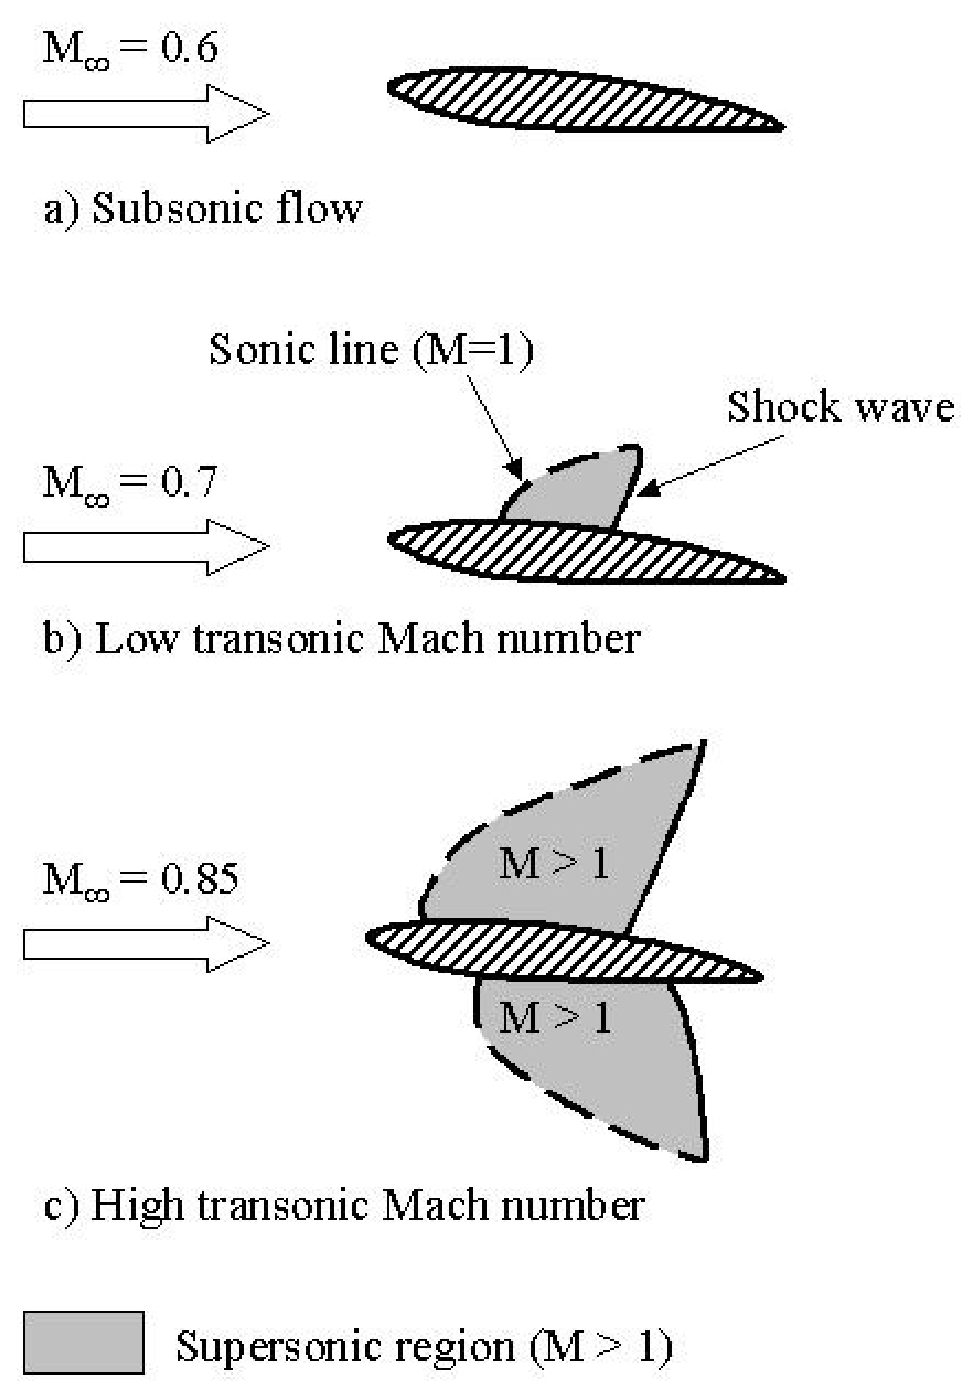
\includegraphics[height=6in]{aflow}
%%%%     \else
%%%%       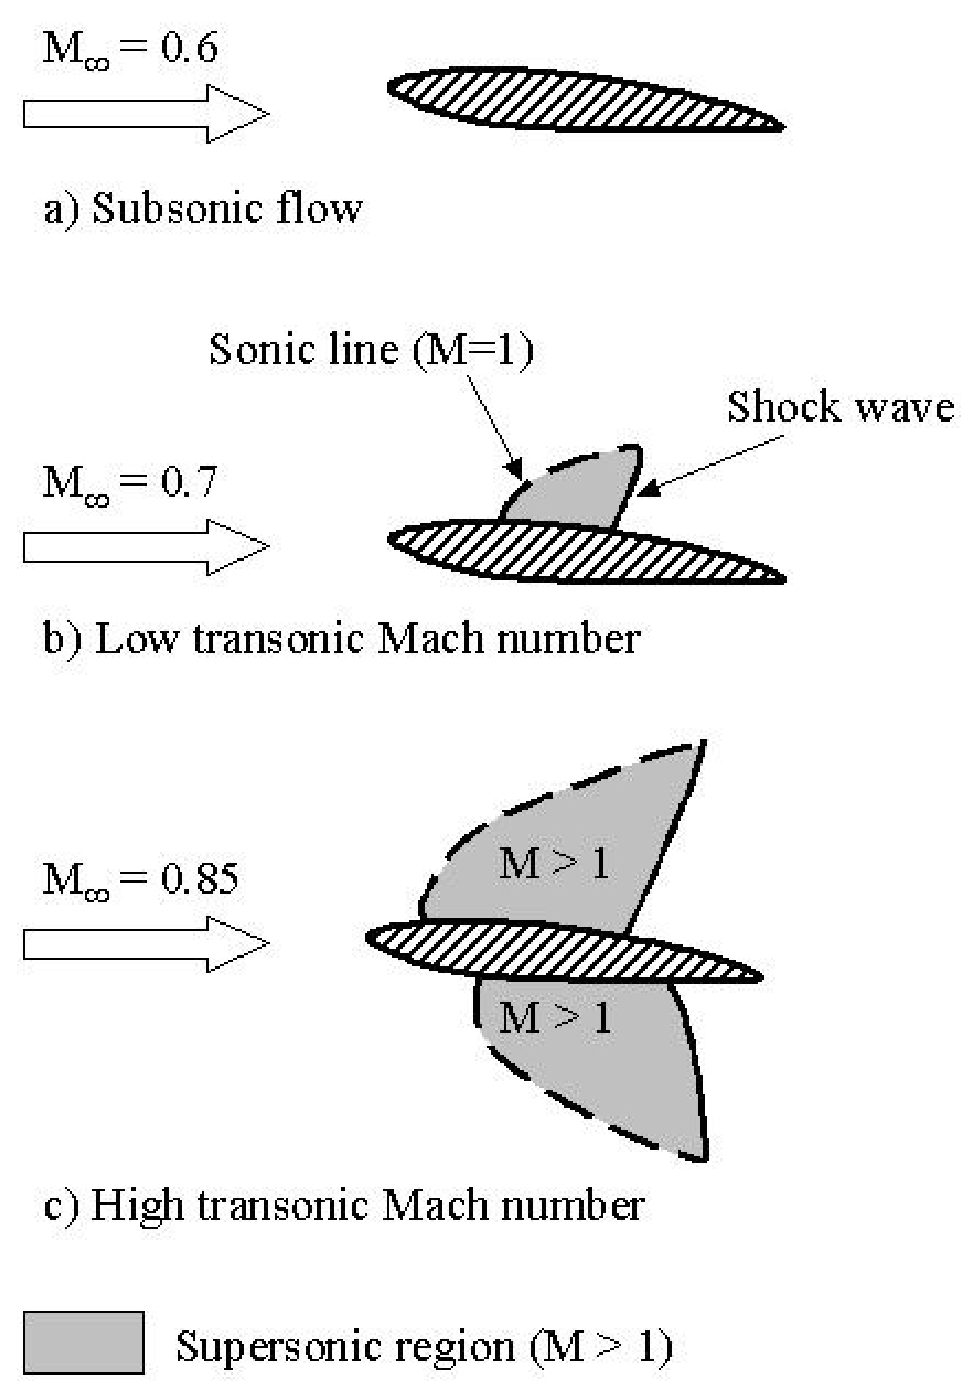
\includegraphics[bb = 92 86 545 742, height=6in]{aflow}
%%%%     \fi
%%%%     \caption{Airfoil Picture}
%%%%     \label{FigAir}
%%%%   \end{center}
%%%% \end{figure}
%%%% 
%%%% % above code has been macro-fied in Classes/MacroFile.tex file
%%%% %\InsertFig{\IncludeGraphicsH{aflow}{6in}{92 86 545 742}}{Airfoil Picture}{FigAir}
%%%% 
%%%% So as we have now labelled it we can reference it, like so (\ref{FigAir}) and it
%%%% is on Page \pageref{FigAir}. And as we can see, it is a very nice picture and we
%%%% can talk about it all we want and when we are tired we can move on to the next
%%%% chapter ...
%%%% 
%%%% I would also like to add an extra bookmark in acroread like so ...
%%%% \ifpdf
%%%%   \pdfbookmark[2]{bookmark text is here}{And this is what I want bookmarked}
%%%% \fi
